% Section content template for individual Educative lessons
% This file contains the actual content for a specific section
% Generated from Educative API section content

% Section: Introduction to Distributed System Failures
% Section ID: 6503055815606272
% Section Slug: introduction-to-distributed-system-failures
% Generated: 2025-12-08T15:36:48.647405

\subsection{Introduction}\label{cb_mJdYvboRIP28aQqYFx}
\\
Once in a while, we encounter the failure of a service that's a household name, and individuals and businesses react to them. As system designers, we might wonder how carefully designed services that have been perfected over years by experienced teams can also fail.\\
This chapter discusses some of the major failures of well-known services and the measures that can be taken to mitigate such failures.
\\
The following two factors contribute to failures:

\begin{itemize}
\item
\protect\phantomsection\label{s4fOF43z-H5uivUJXO0Gr}
\textbf{Diverse users}: Most services have a vibrant user community, and as their needs evolve, so do the software products. If a software doesn't update in the way it provides new features and services, it will become stable over time. However, it might not have the features customers want.
\item
\protect\phantomsection\label{dOp74EPhhCalYTpc_JiOU}
\textbf{Complex systems}: Systems are complex, and they usually have emergent properties where the sum of system components is more complex than the individual pieces.
\end{itemize}

% \vspace{-1.0\baselineskip}
\noindent
\begin{minipage}[t]{0.48\textwidth}\vspace{0pt}

\end{minipage}
\hfill
\begin{minipage}[t]{0.48\textwidth}\vspace{0pt}

\end{minipage}

\begin{figure}[htbp]
 \centering
 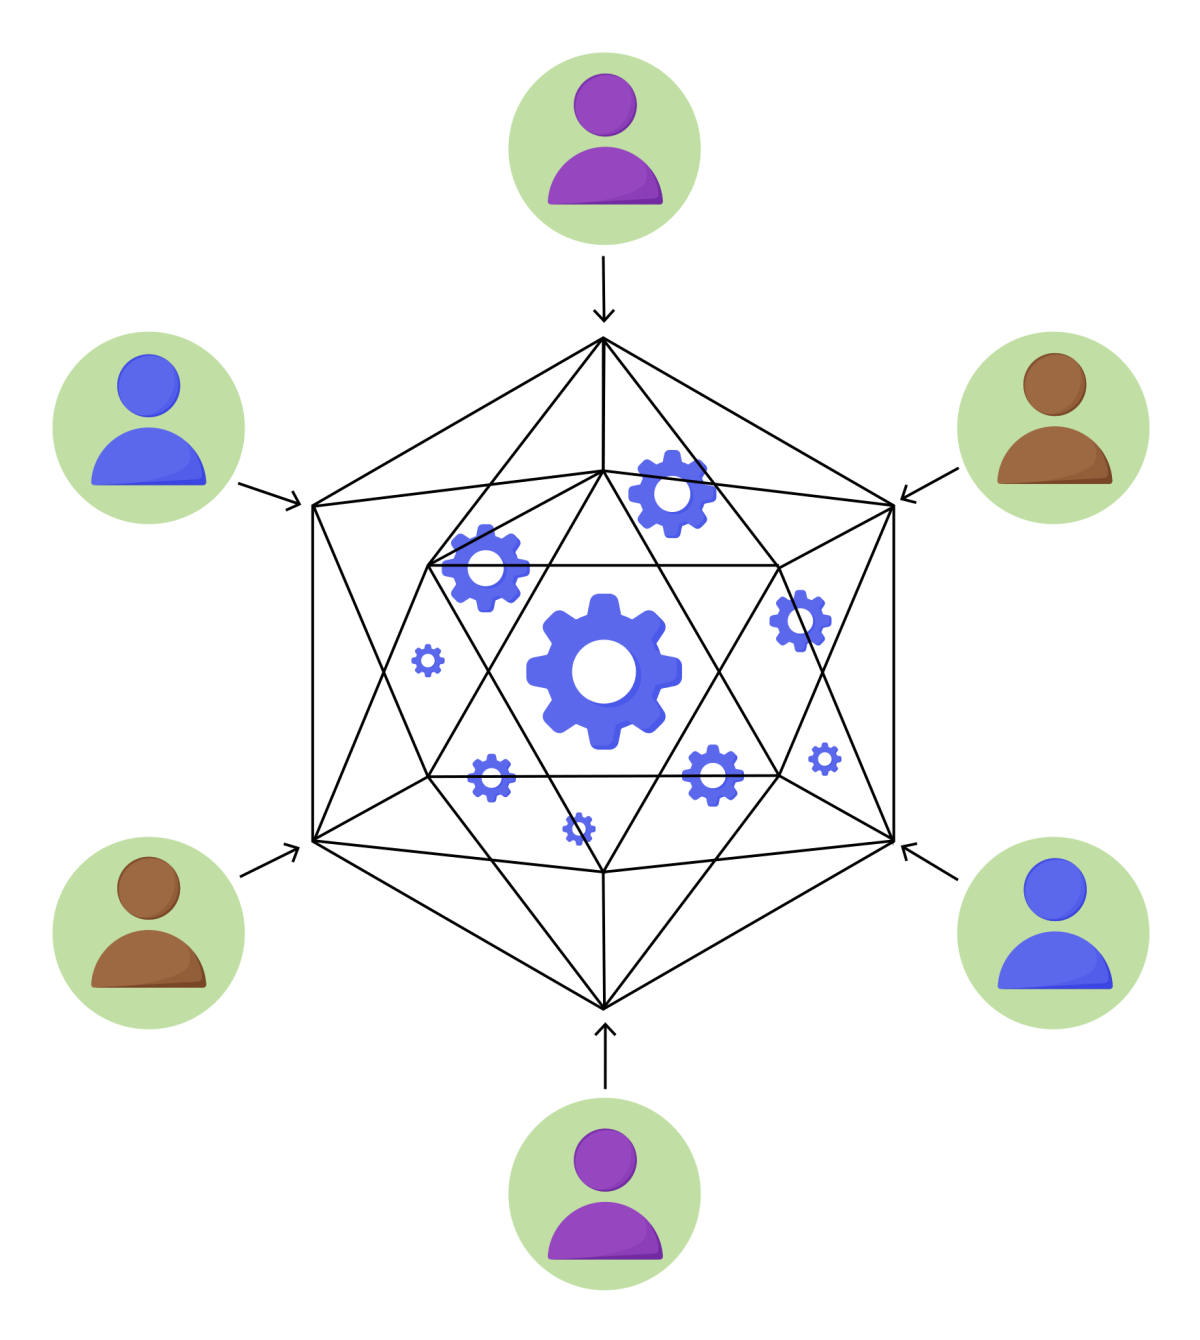
\includegraphics[width=0.25\textwidth]{Images/chapter_42/section_6503055815606272/4705583079751680.png}
 \caption{Diverse users interacting with a complex system}
\end{figure}

\subsection{Types of failure in distributed systems}\label{UmU0WmPcFyJEHMXiiv0bJ}
\\
Most modern services are designed in such a way that failures are contained, and others might be localized for some users. Let 's explore the types of failures we can observe in the distributed systems.

\begin{itemize}
\item
\protect\phantomsection\label{Mrn_itJ87GSu8fRfemGyT}
\textbf{System failure}: A software or hardware failure is the most common cause of system failure. The contents in the primary memory are lost when a system fails. However, the data in secondary storage or replicas remains unaffected. The system reboots during such a breakdown.
\item
\protect\phantomsection\label{hJU0ZKpSODKlfGBy9Bhym}
\textbf{Method failure}: Such failures suspend the working of distributed systems. It may also make the system execute the processes incorrectly or enter a deadlock state.
\item
\protect\phantomsection\label{7pfRLeBq0K1dexaA09_Pt}
\textbf{Communication medium failure}: Such failures occur when one component or service of a system can't reach the other internal or external entities.
\item
\protect\phantomsection\label{246AAXECm4nla_7ZAwlnq}
\textbf{Secondary storage failure}: In such failures, the secondary storage or replicas are down. The data in these nodes becomes inaccessible, so primary nodes need to generate another replica to ensure reliability and fault tolerance.
\end{itemize}

\begin{figure}[htbp]
 \centering
 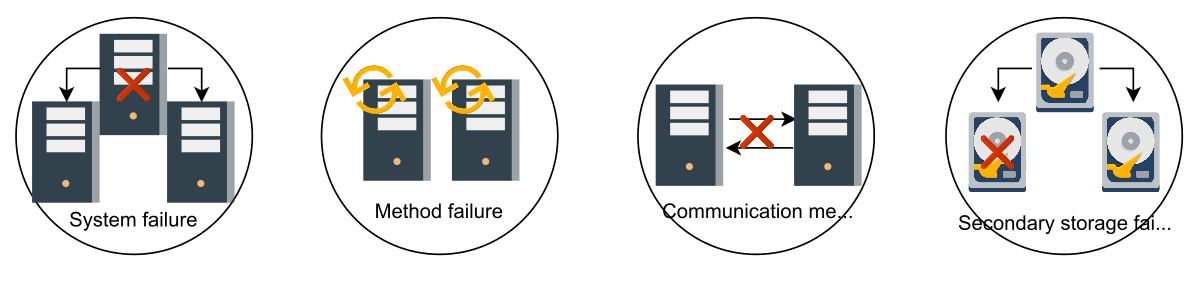
\includegraphics[width=0.5\textwidth]{Images/chapter_42/section_6503055815606272/5696385278279680.png}
 \caption{Types of failure in a distributed system}
\end{figure}

\subsection{Vantage points}\label{O8qVDbRZ6f71EMMrddezh}
\\
Something is always failing for large services. It 's preferred to have a graceful degradation so that only a small portion of users are impacted for a short time. Therefore, we need globally dispersed vantage points to independently see the service status.
\begin{quote}
\textbf{Note:} Many independent services, such as Downdetector, exist for crowd-sourced problem reporting. It's interesting to note that if we visit such a service and see the status of our favorite applications, we'll see that there's always someone in the world facing some service problem.
\end{quote}
\subsubsection{Importance of independent service providers}\label{RAwvEaum2ibhDbjNS5XlJ}
\\
One of the design goals of the original Internet was to provide resilience so that if one part fails, the rest can still operate.
\\
With the emergence of a handful of service providers over the last decade, critics have raised concerns(See ``It's time to decentralize the internet, again: What was distributed is now centralized by Google, Facebook, etc'' by Bruce Davie.) about such centralization and the potential impacts of failures. Most companies provide some kind of dashboard to enable users to see the service status.
\\
However, some failures might even knock out these dashboards. Affected companies then communicate to their customers via services like Twitter to announce the updates. Independent third-party services are valuable for failure detection and status dissemination.
\begin{quote}
\textbf{Note:} The broader concept here is to use independent failure domains. A \textbf{failure domain} is a concept where anything failing inside a domain or network shouldn't affect other components and services in other domains. At times, we say that two domains are independent if they're outside the blast radius of each other.
\end{quote}

\begin{figure}[htbp]
 \centering
 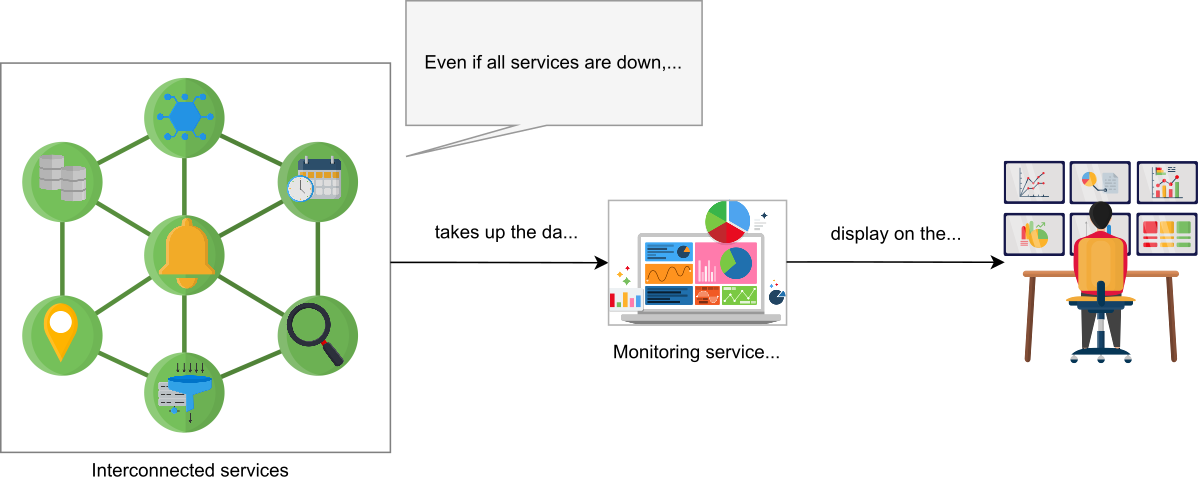
\includegraphics[width=0.5\textwidth]{Images/chapter_42/section_6503055815606272/5958544713318400.png}
 \caption{Importance of independent service}
\end{figure}

In the following lessons, we'll discuss the failures of well-known services by giant companies, the causes of failures, and what mitigation techniques can be used to avoid these failures. Although failures are a great way to learn what went wrong and what the original designers could do to avoid such failures, we'd like to prevent them from occurring at all.

% End of section content